\documentclass[12pt, titlepage]{article}

\usepackage{graphicx} % Allows for images
\usepackage{wrapfig} % Allows for text wrapping around images
\usepackage{hyperref} % Allows for hyperlinks
\usepackage{siunitx} % Allows for SI units
\usepackage{amsmath} % Allows for math
\usepackage{enumerate} % Allows for custom enumerations
\usepackage{xcolor} % Allows for custom colors
\usepackage{tikz, tcolorbox} % Allows for custom boxes
\usepackage{microtype} % Allows for better text alignment
\usepackage{listings} % Allows for code listings
\usepackage{booktabs} % Allows for better tables
\usepackage{float} % Allows for better figure placement
\usepackage{geometry} % Allows for custom page geometry
\usepackage{fancyhdr} % Allows for custom headers and footers
\usepackage{caption} % Allows for custom captions

\fancypagestyle{myarticlestyle}{
  \fancyhf{} % Clear header and footer
  \fancyhead[L]{\leftmark} % Section name on the left
  \fancyhead[R]{\thepage} % Page number on the right
}
\fancypagestyle{tocstyle}{
  \fancyhf{} % Clear header and footer
  \fancyhead[L]{CONTENTS} % Section name on the left
  \fancyhead[R]{\thepage} % Page number on the right
}

\pagestyle{myarticlestyle}
\setlength{\headheight}{15pt}

\title{Heat Exchanger Design MATLAB Assignment}
\author{Omar Ebrahim\footnote{The signature can be found in the last page of
this document} 110076575\\ebrahimo@uwindsor.ca\\Dr. Randy Bowers\\ University
of Windsor}

\begin{document}
\maketitle
\tableofcontents
\listoffigures
\newpage
\section{Results}
The following are the results of the MATLAB code. The data ledger is shown in
Figure \ref{fig:ledger}. The data ledger shows the data for the inlet temperature,
mass flow rate of water from constant specific heat, mass flow rate of water from
saturated liquid water interpolation.
\begin{figure}[H]
  \centering
  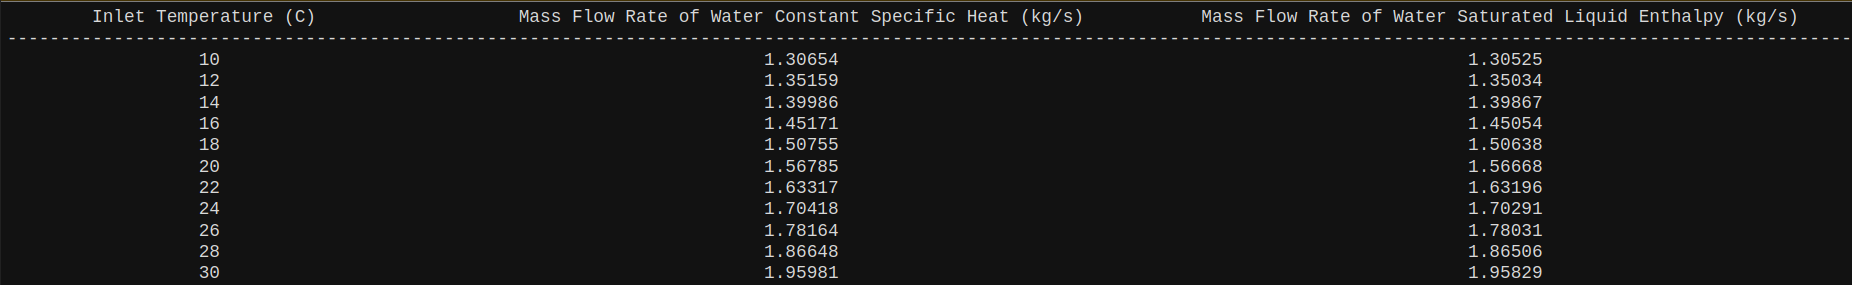
\includegraphics[width=1\textwidth]{../data_ledger.png}
  \caption{Data ledger}
  \label{fig:ledger}
\end{figure}
The graphs of the inlet temperature vs the mass flow rate of water from constant
specific heat and mass flow rate of water from saturated liquid water interpolation
are shown in Figure \ref{fig:graphs}. The blue line represents the mass flow rate
of water from constant specific heat and the red line represents the mass flow
rate of water from saturated liquid water interpolation.
\begin{figure}[H]
  \centering
  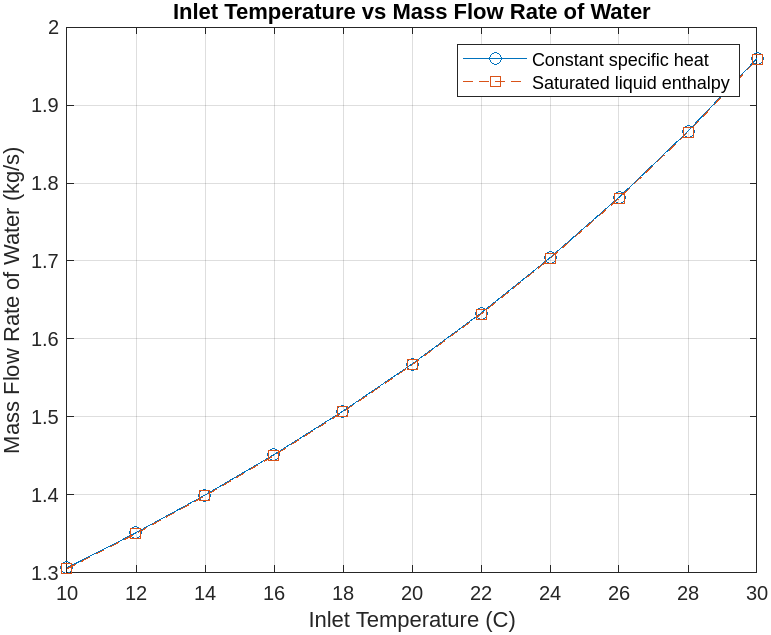
\includegraphics[width=0.63\textwidth]{../graph.png}
  \caption{Graphs of the inlet temperature vs the mass flow rate of water from
  constant specific heat and mass flow rate of water from saturated liquid water
  interpolation}
  \label{fig:graphs}
\end{figure}
\section{Range}
This section will calculate the range of the mass flow rates of water from constant
specific heat and mass flow rate of water from saturated liquid water interpolation.
The range of the mass flow rates can be found using the following equation:
\begin{equation}
  \text{Range} = \text{Maximum} - \text{Minimum}
  \label{eq:range}
\end{equation}
First calculate the range of the mass flow rate of water from constant specific
heat. Putting the values from the data ledger into Equation \ref{eq:range} gives:
\begin{align}
  \text{Range} &= 1.95981 - 1.30654 \nonumber \\
  &= 0.65327
  \label{eq:range_constant_specific_heat}
\end{align}
Now calculate the range of the mass flow rate of water from saturated liquid water
interpolation. Putting the values from the data ledger into Equation \ref{eq:range}
gives:
\begin{align}
  \text{Range} &= 1.95829 - 1.30525 \nonumber \\
  &= 0.65304
  \label{eq:range_saturated_liquid_water_interpolation}
\end{align}
Therefore, the range of the mass flow rates of water from constant specific heat
and mass flow rate of water from saturated liquid water interpolation are 0.65327
and 0.65304 respectively.
\section{Variance}
As shown in Figure \ref{fig:ledger}, the data from the mass flow rate of water
from constant specific heat and the mass flow rate of water from saturated liquid
water interpolation are very similar. The differences between the two data sets
mostly starts at the the third decimal place. Therefore, there is not much variance
between the two data sets.
\section{Percent Error}
To find the percent error, calculate the average of the mass flow rate of water
from constant specific heat and the mass flow rate of water from saturated liquid
water interpolation. The average of the mass flow rate of water from constant
specific heat is found using the following equation:
\begin{equation}
  \bar{m}_{\text{constant specific heat}} = \frac{1}{n}\sum_{i=1}^{n}m_i
  \label{eq:average_constant_specific_heat}
\end{equation}
Putting the values from the data ledger into Equation
\ref{eq:average_constant_specific_heat} gives:
\begin{align}
  \bar{m}_{\text{constant specific heat}} &= \frac{1}{11}(1.30654 + 1.35159 + 1.39986 + 1.45171 + 1.50755 \nonumber \\
  &\quad + 1.56785 + 1.63317 + 1.70418 + 1.78164 + 1.86648 + 1.95981) \nonumber \\
  &= 1.5937
  \label{eq:average_constant_specific_heat_values}
\end{align}
The average of the mass flow rate of water from saturated liquid water interpolation
is found using the following equation:
\begin{equation}
  \bar{m}_{\text{saturated liquid water interpolation}} = \frac{1}{n}\sum_{i=1}^{n}m_i
  \label{eq:average_saturated_liquid_water_interpolation}
\end{equation}
Putting the values from the data ledger into Equation
\ref{eq:average_saturated_liquid_water_interpolation} gives:
\begin{align}
  \bar{m}_{\text{constant specific heat}} &= \frac{1}{11}(1.30525 + 1.35034 + 1.39867 + 1.45054 + 1.50638 \nonumber \\
  &\quad + 1.56668 + 1.63196 + 1.70291 + 1.78031 + 1.86506 + 1.95829) \nonumber \\
  &= 1.5924
  \label{eq:average_saturated_liquid_water_interpolation_values}
\end{align}
Now that the averages are found, the percent error can be calculated using the
following equation:
\begin{equation}
  \text{Percent Error} = \left| \frac{\text{Experimental Value} - \text{Theoretical Value}}{\text{Theoretical Value}}\right| \times 100\%
  \label{eq:percent_error}
\end{equation}
Assuming that the mass flow rate of water from saturated liquid water interpolation
is the theoretical value and the mass flow rate of water from constant specific
heat is the experimental value.\\[10pt]
Putting the values from Equations
\ref{eq:average_constant_specific_heat_values} and
\ref{eq:average_saturated_liquid_water_interpolation_values} into Equation
\ref{eq:percent_error} gives:
\begin{align}
  \text{Percent Error} &= \left| \frac{1.5937 - 1.5924}{1.5924}\right| \times 100\% \nonumber \\
  &= 0.000816 \times 100\% \nonumber \\
  &= 0.0816\%
  \label{eq:percent_error_values}
\end{align}
Therefore, the percent error of the mass flow rates of water is 0.0816\%.
\section{Sources of Error}
The sources of error are the assumptions made in the MATLAB code. The first
assumption is that the specific heat of water is constant. This is not true
because the specific heat of water changes with temperature. The second assumption
is that the mass flow rate of water from saturated liquid water interpolation
is accurate. The interpolation can be inaccurate because the interpolation is
approximating the data using lines which may or may not accurately represent the
data.
\section{Conclusion}
This report concludes with the following:
\begin{enumerate}
  \item The range of the mass flow rates of water from constant specific heat
  and mass flow rate of water from saturated liquid water interpolation are 0.65327
  and 0.65304 respectively.
  \item The variance between the mass flow rate of water from constant specific
  heat and the mass flow rate of water from saturated liquid water interpolation
  is very small.
  \item The percentage error of the mass flow rates of water is 0.0816\%.
  \item The sources of error are the assumptions made in the MATLAB code. The first
  assumption is that the specific heat of water is constant. This is not true
  because the specific heat of water changes with temperature. The second assumption
  is that the mass flow rate of water from saturated liquid water interpolation
  is accurate. The interpolation can be inaccurate because the interpolation is
  approximating the data using lines which may or may not accurately represent the
  data.
\end{enumerate}
\newpage
\begin{figure}[H]
  \centering
  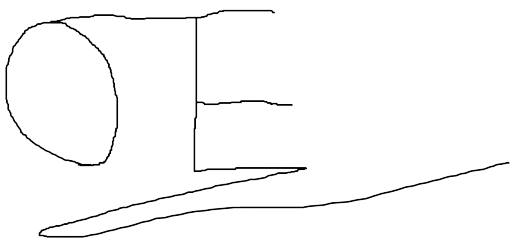
\includegraphics[width=1\textwidth]{./Images/signature.png}
\end{figure}
\end{document}
% End of report.tex
